\section{Implementation and Experimental Results}
\label{sec:genomics-experimental}

In this section we present experimental results for our protocols for
computing the edit distance and the Smith-Waterman distance between
two strings.  For edit distance, our tests were performed on random
strings.  For the Smith-Waterman distance, we aligned representative protein
sequences from the Pfam database of protein sequences~\cite{pfam2002}
in protein family {\sf QH-AmDH\_gamma (PF08992)}, which is a
crystalline quinohemoprotein amine dehydrogenase from Pseudomonas
putida.  The average length of these proteins is 78 amino acids.  In
order to demonstrate the scalability of the algorithm, we truncate the
proteins to various lengths as shown in figure 6.  For a cost
function, we used the BLOSUM62 matrix~\cite{blosum62} which is a
$(20,20)$ substitution matrix based on log-odds statistics derived
from experimental protein data which approximates the probability of
substitution of amino acids in homologous proteins.  It is a commonly
used metric in genomic research.

\subsection{Edit distance}

% In this section, we describe our implementation of the three protocols
% for privately computing the edit distance between two strings and present
% experimental results for network bandwidth and execution times.

We implemented the standard methods for secure circuit evaluation,
\ie, the Yao's ``garbled circuits'' method and secure computation with
shares (see sections \ref{sub:Garbled-Circuit-Method} and \ref{sub:SCWS}).  We used the oblivious transfer
protocol due to Noar and Pinkas (see section~\ref{sub:Oblivious-Transfer}).  For the
minimum-of-three computation, we used the lowest price auction circuit of
Kurosawa and Ogata~\cite{KO02}.  Using these primitives, we implemented
the three protocols of section~\ref{sec:protocols}.  For comparison
purposes, we also implemented the edit distance protocol of Atallah
\textit{et al.}~\cite{atallah}, using the Lin-Tzeng construction for
the millionaires' protocol~\cite{lintzeng-acns05} and Paillier homomorphic
encryption~\cite{Paillier99} (see section~\ref{appendix-atallah}).
All of the code was written in Java.

The experiments were executed on two 3-GHz Pentium 4 machines, with two
gigabytes of memory, and connected via a local LAN. Using this setup,
we obtained measurements (network bandwidth and execution times) for
the three protocols on various problem sizes. The reason for performing
the experiment on a local LAN is to provide a ``best-case'' result
for execution times in an environment where network bandwidth is not
a bottleneck.  Because the bandwidth numbers presented do not depend on
the experimental setup, execution times for bandwidth-limited networks
can be estimated from the numbers presented here.

The size of the problem instance is $(n,m)$, where $n$ and $m$
are the sizes of the two strings. For simplicity, all experiments
were performed on problems where $m=n$. The main conclusions that
can be drawn from our measurements are:

\begin{itemize}

\item \textit{Protocol 1 is not suitable for large problems.} 
Protocol 1 is ideal for small strings because the entire computation is
performed in one round, but the circuit size is extremely large for longer
strings.  We exhausted all available memory on our experimental machine
when evaluating a circuit for a problem instance of size $(26,26)$.

\item \textit{Protocol 2 can execute for problems of any size.} 
Protocol 2 performs reasonably well for moderate-size instances.
For example, a problem of size $(100,100)$ takes just under $9$ minutes
in our experimental setup.  Protocol 1 cannot scale to problems of
this size (although it is more efficient for very small problems).


\item \textit{Protocol 3 is most suitable for large problems.} 
Protocol 3 uses the grid structure of the problem space, which makes it
most suitable for large instances.  For example, a problem instance of
size $(200,200)$ takes under 10 minutes.  Asymptotically, protocol 3 has
the same performance as protocol 2, but in practice it is substantially
faster.  
\item \textit{Bandwidth requirements are asymmetrical.} 
Bandwidth requirements are asymmetrical.  Because Alice sends the
majority of data in the Naor-Pinkas~\cite{Naor-Pinkas:2001} oblivious
transfer protocol, bandwidth requirements are asymmetrical.
Specifically, Alice sends far more data than she receives and vice
versa for Bob.  This is useful because many real world communications
channels, such as ADSL or cable lines, offer a greater bandwidth for
transmitting data in one direction than in the other.  In this case,
the protocol would run with greater speed by assigning Alice's role to
the party that sends data faster, and Bob's role to the party that
receives data faster.


\item \textit{The edit distance protocol by Atallah et al.~\cite{atallah}
is not practical.} 
In our experiments, the protocol of~\cite{atallah} performed at least an
order of magnitude worse than our protocols.  This is because many large
numbers (Paillier ciphertexts) are computed and sent multiple times by
both Alice and Bob at each step.  For example, on problem instance of
size $(25,25)$ the protocol by Atallah \textit{et al.} took $5$ and half
minutes.  Our Protocol $3$ took $14$ seconds on the same problem instance.

\end{itemize}

Figure~\ref{fig:histogram} shows the execution times for our three
protocols. Clearly, protocol $3$ scales the best as the problem size
increases. Protocol $1$ is suitable for small problems. Protocol $2$
has a larger execution time, but only requires limited bandwidth per
round. Our experimental results confirm the protocol characteristics
shown in Figure~\ref{fig:protocol-characteristics}.

\begin{figure*}
\centerline{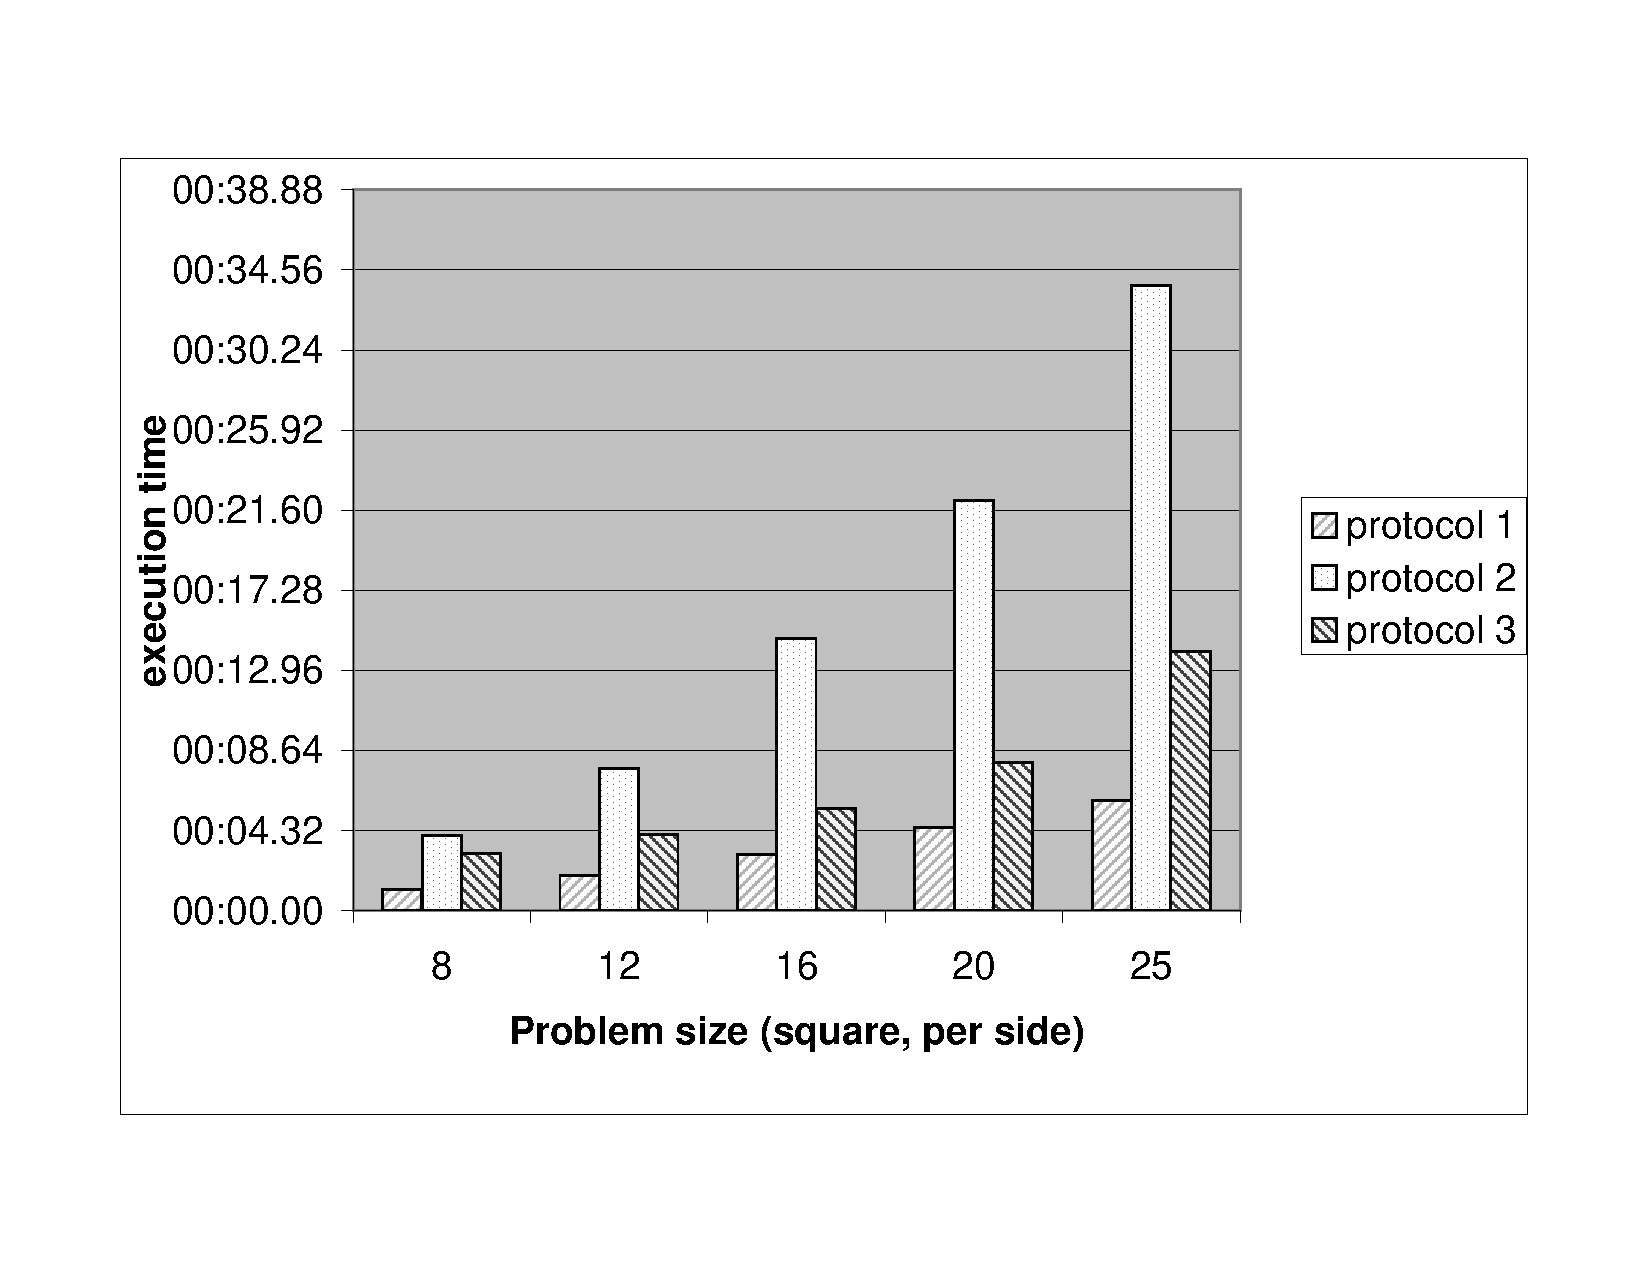
\includegraphics[bb=22bp -50bp 600bp 1000bp,scale=0.6,angle=0]{genomics/proto123}}
\caption{Timing measurements (in minutes and seconds) comparing protocols
1, 2, and 3. The Atallah~\cite{atallah} protocol could not complete problems of
sizes $(25,25)$ and $(25,25)$.}
\label{fig:histogram} 
\end{figure*}

Detailed results for protocol $1$ and $2$ are presented in section~\ref{appendix-atallah}.
We discuss here results for Protocol $3$ in detail. Recall that
in this protocol a grid structure is used (see
section~\ref{subsec:protocol3}).  Using Protocol $3$, we were able to
solve problems instances of considerable size; here we present
measurements for a problem instance of size
(200,200). Table~\ref{protocol3table200} shows the results using
various grid sizes. Performance steadily improves up to the grid size
of $20$, but begins to decrease slightly after that.  In spite of
decreased overall performance, further increases in the grid size
slightly decrease network bandwidth requirements, which results in
fewer round trips, so even larger grid sizes may be suitable for
environments with limited network bandwidth.  With a grid size of
$20$, Protocol 3 requires about as much time for an instance of size
$(200,200)$ as Protocol 2 requires for an instance of size ($25,25)$.


\subsection{Smith-Waterman}
\label{sec:sw-experimental}

For Protocols 1 and 3, the Yao circuit is modified by embedding the
cost function in the circuits. Recall that for edit distance, $\sigma=0$
if $\alpha[i]=\beta[j]$, $1$ otherwise. In Smith-Waterman, $\sigma$ is
an arbitrary cost function $c(u,v)$. The modified circuits effectively
perform a table lookup on $c(\alpha[i],\beta[j])$ in determining the
lowest cost alignment. Likewise, the gap function, which is a constant $1$
for edit distance, is replaced by the gap value of the scoring function
for Smith-Waterman. By convention, lower numbers represent higher costs
(higher numbers represent a similarity score) so a maximum-of-three circuit is
used instead of min-of-3.

We also constructed a protocol for Smith-Waterman based on Protocol
2. Recall that in Protocol $2$ for edit distance, a circuit for
equality of the characters is evaluated. For Smith-Waterman, an
$OT_1^{\mid \Sigma \mid}$ is performed instead. Alice, acting as the sender,
creates an array with a row of the cost function subtracted from her
random share $r$.  Each element of the array is $r-c(\alpha[i],\beta)$
for each possible $\beta\in\Sigma$. Bob, acting as the chooser, selects
the element with index $\beta[j]$. In this way, Bob receives the value
$r-c(\alpha[i],\beta[j])$.  Alice and Bob's shares are then input into
a maximum-of-three circuit which computes the next value of the shared dynamic
programming matrix.  The remaining details of the protocol are the same
as for edit distance.


Figure~\ref{fig:sw-histogram} shows the timing measurements for the
three protocols.  For Protocols 1 and 3, the computation time scales
with the size of the score matrix, which is ${\mid \Sigma \mid}^{2}$. For
example, the bytes transferred over the network aligning protein
sequences using BLOSUM62 are approximately 40 times that of for simple
edit distance of the same size problem.  This is caused by the use of
extra gates in the Yao circuit which encode each value of the score
function.  For Protocol 2, the computation scales with the alphabet
size $\mid \Sigma \mid$. For a very large alphabet with hundreds of symbols,
Protocol $2$ would be the best choice because the cost of embedding
the entire matrix into a Yao circuit becomes prohibitive.

\begin{figure*}
\centerline{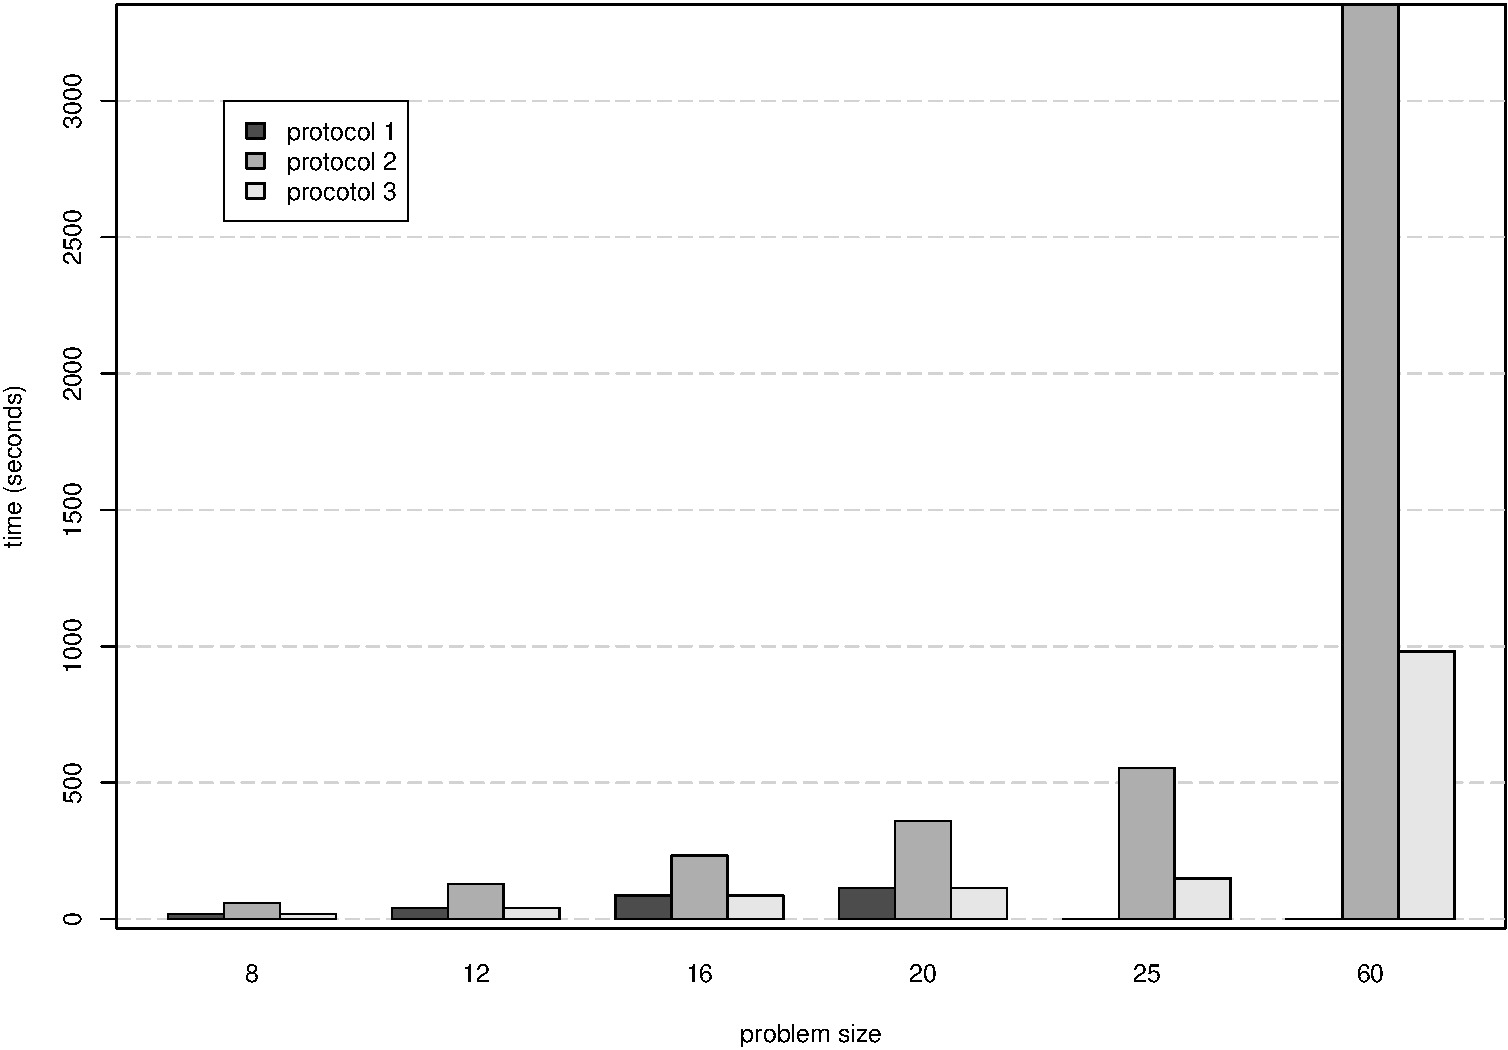
\includegraphics[scale=0.6,angle=0]{genomics/sw123}}

\caption{Timing measurements (in minutes and seconds) comparing Smith-Waterman
Protocols 1, 2, and 3. For problem sizes (25,25) and (60,60), Protocol
1 could not evaluate the circuit.}

\label{fig:sw-histogram} 
\end{figure*}

\begin{table}
\begin{centering}
\begin{tabular}{|c||c|c|c|c|c|}
\hline 
Grid size &
Bandwidth (Alice) &
Bandwidth (Bob) &
CPU (Alice) &
CPU (Bob) &
wall clock \tabularnewline
\hline
\hline 
25 &
362.2 M &
2.1 M &
518 &
84 &
658 \tabularnewline
\hline 
20 &
368.5 M &
2.6 M &
385 &
90 &
534 \tabularnewline
\hline 
10 &
397.4 M &
5.4 M &
476 &
123 &
655 \tabularnewline
\hline 
8 &
412.0 M &
5.8 M &
520 &
145 &
729 \tabularnewline
\hline 
4 &
485.3 M &
14.4 M &
784 &
234 &
1095 \tabularnewline
\hline 
2 &
635.2 M&
32.0 M&
1296 &
408 &
1804 \tabularnewline
\hline 
1&
948.0 M&
76.7 M&
2480 &
780 &
4883 \tabularnewline
\hline
\end{tabular}
\par\end{centering}

\caption{Network bandwidth (in bytes) and timing measurements (in seconds)
for edit-distance Protocol 3 with a problem of size $(200,200)$.
(M refers to Megabytes)}

\label{protocol3table200} 
\end{table}




